\documentclass[tikz,border=4pt]{standalone}
\usepackage{fontspec}
\setmainfont{Liberation Serif}
\usepackage{pgfplots}
\pgfplotsset{compat=1.18}
\begin{document}
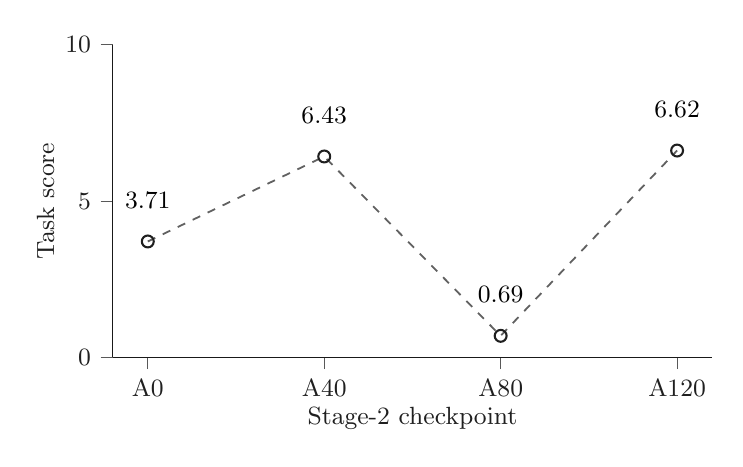
\begin{tikzpicture}
\begin{axis}[
  width=9.2cm,height=5.55cm,
  xmin=-8,xmax=128,ymin=0,ymax=10,
  xtick={0,40,80,120},
  xticklabels={A0,A40,A80,A120},
  ytick={0,5,10},
  xlabel={Stage-2 checkpoint},
  ylabel={Task score},
  axis x line*=bottom,
  axis y line*=left,
  tick align=outside,
  tick style={line width=0.35pt,color=black!65},
  axis line style={line width=0.55pt,color=black!90},
  tick label style={font=\small,color=black!88},
  label style={font=\small,color=black!88},
  xlabel style={yshift=1mm},
  ylabel style={yshift=-1mm},
  grid=none,
  clip=false,
]
\addplot+[
  no markers,
  color=black!62,
  line width=0.65pt,
  dashed
] coordinates {(0,3.71)(40,6.43)(80,0.69)(120,6.62)};
\addplot+[
  only marks,mark=o,mark size=2.15pt,
  mark options={color=black!88,fill=white,line width=.75pt}
] coordinates {(0,3.71)(40,6.43)(80,0.69)(120,6.62)};
\node[above=3.0mm,font=\small,text=black] at (axis cs:0,3.71) {3.71};
\node[above=3.0mm,font=\small,text=black] at (axis cs:40,6.43) {6.43};
\node[above=3.0mm,font=\small,text=black] at (axis cs:80,0.69) {0.69};
\node[above=3.0mm,font=\small,text=black] at (axis cs:120,6.62) {6.62};
\end{axis}
\end{tikzpicture}
\end{document}
